%%----------------------------------------------------------------------------------------
\clearpage
\pagestyle{fancy}
%%----------------------------------------------------------------------------------------
%%       PREFAZIONE
%%----------------------------------------------------------------------------------------
\part{Il diagramma di $M$ in un tratto rettilineo su cui agisce un carico trasversale uniforme}
\setcounter{section}{0}
%----------------------------------------------------------------------------------------
Abbiamo già dimostrato che, nel caso in questione, il diagramma di $M$ è una \textbf{parabola}; ci proponiamo di fornire un procedimento atto a costruirla, in maniera quanto meno \emph{decente}. Consideriamo, a titolo di esempio, la trave in figura~\ref{figura14-1}. Trovate le reazione vincolari, abbiamo disegnato il diagramma di $M$ come se, invece di $q$, vi fosse la sua risultante concentrata; si tratta della spezzata $HKIJ$, essendo l'ordinata di $K$ pari a $\frac{3}{8}qL \cdot \frac{L}{4} = \frac{3}{32} qL^{2}$. La parte $HKI$ è tratteggiata perché essa \textsc{non è il vero diagramma di} $M$, mentre la parte $IJ$ lo è. Tuttavia, le rette $HK$ e $KI$ sono utili ai fini di costruire il vero diagramma di $M$: non è difficile dimostrare che esse sono le tangenti alla parabola, rispettivamente, nei punti $H$ ed $I$, considerato che i \textsc{tagli}, cioè le derivate di $M$, \textbf{sono gli stessi sia nel caso in vi è} $q$, \textbf{sia nel caso in cui vi è la risultante concentrata}. Per questo motivo, le tangenti in $A$ ed in $B$ ai diagrammi di $M$ coincideranno nei casi del carico distribuito e della sua risultante concentrata. Disporre delle tangenti alla parabola ai due estremi è utile ai fini di poterla disegnare correttamente, ma c'è di più: detti $1$ e $2$ i punti medi dei segmenti $HK$ e $KI$, la retta che li congiunge è anch'essa tangente alla parabola esattamente nel punto $T$, intersezione della linea $12$ con la retta d'azione della risultante del carico. A questo punto la parabola si può disegnare. Tuttavia, è interessante sottolineare le seguenti circostanze, che possono talvolta risultare preziose e la cui dimostrazione è lasciata al lettore: 
%----------------------------------------------------------------------------------------
\begin{enumerate}
\item la retta $12$ è parallela alla congiungente $HI$; 
\item $T$ è il punto medio del segmento $LK$; 
\item si può vedere che vale la seguente 
	\begin{equation*}
		\big| LK \big| = \frac{ \text{Carico} \times \text{Lunghezza}^{2} }{ 4 }
	\end{equation*}
si noti che in figura~\ref{figura14-1} risulta $\big| LK \big| = \frac{qL^{2}}{16}$.
\end{enumerate}
%----------------------------------------------------------------------------------------
%--------------------------------------------------------------------------------------------------------------------------------------------------------------
\renewcommand{\thefigure}{14~-~1}
\begin{figure}[ht]
\centering
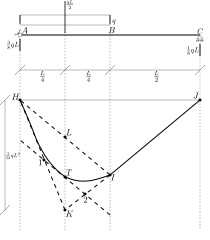
\includegraphics[width=0.95\textwidth]{Immagini/Parte_14/Figura14_1/figura14_1.pdf}
\caption{}
\label{figura14-1}
\end{figure}
%--------------------------------------------------------------------------------------------------------------------------------------------------------------